% 8239a118-9287-4621-93a2-5e67160bc619
\documentclass{article}
\usepackage[utf8]{inputenc}
\usepackage{multicol}
\usepackage{listings}
\usepackage{amssymb}
\usepackage{amsfonts}
\usepackage{amsmath}
\usepackage{enumitem}
\usepackage{graphicx}
\usepackage{amsthm}
\usepackage{hyperref}
\usepackage{tikz}
\usetikzlibrary{arrows}
\usepackage[ruled,vlined]{algorithm2e}
\newtheorem{theorem}{Theorem}
\newtheorem{definition}{Definition}

\SetKwFunction{dijkstraAirlines}{dijkstraAirlines}
\SetKwProg{Fn}{Function}{}{}
\SetKwProg{Proc}{Procedure}{}{}

%=====================================
%			Assignment 4
%=====================================

\begin{document}

\title{Weekly Assignment 4}
\date{28th September 2017}
\author{Tony Lopar s1013792}
\maketitle

\paragraph{Deadline:} 4th October 2017, 6pm.
\paragraph{Solutions can be found below the exercises}



\section*{Exercise 1.}
From elements $1$, $4$, $7$ and $9$, draw all possible heaps.

\subsection*{Solutions exercise 1}
Since a type of heap is not specified, I will show all the possible min-heaps and all the possible max-heaps. The min-heaps are shown in the top row and the max heaps are shown in row below. \\
\begin{center}
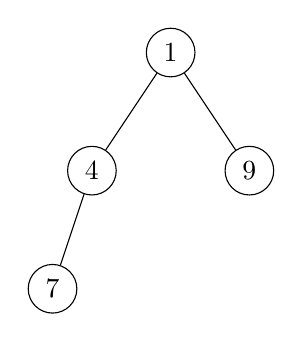
\begin{tikzpicture}[-, level/.style={sibling distance = 2cm/#1, level distance = 1.5cm}, scale=1,transform shape]
    \node[circle,draw](z){$1$}
        child{
            node[circle,draw]{4}
            child{
                node[circle,draw] {7}
                child[missing]
            }
            child[missing]
        }
        child{
            node[circle,draw]{9}
            child[missing]
        };
\end{tikzpicture}
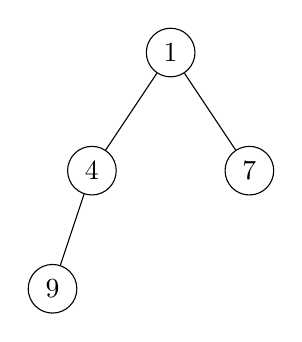
\begin{tikzpicture}[-, level/.style={sibling distance = 2cm/#1, level distance = 1.5cm}, scale=1,transform shape]
    \node[circle,draw](z){$1$}
        child{
            node[circle,draw]{4}
            child{
                node[circle,draw] {9}
                child[missing]
            }
            child[missing]
        }
        child{
            node[circle,draw]{7}
            child[missing]
        };
\end{tikzpicture}
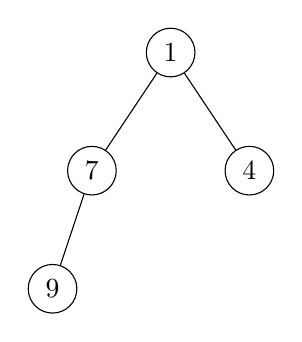
\begin{tikzpicture}[-, level/.style={sibling distance = 2cm/#1, level distance = 1.5cm}, scale=1,transform shape]
    \node[circle,draw](z){$1$}
        child{
            node[circle,draw]{7}
            child{
                node[circle,draw] {9}
                child[missing]
            }
            child[missing]
        }
        child{
            node[circle,draw]{4}
            child[missing]
        };
\end{tikzpicture}
\end{center}
\begin{center}
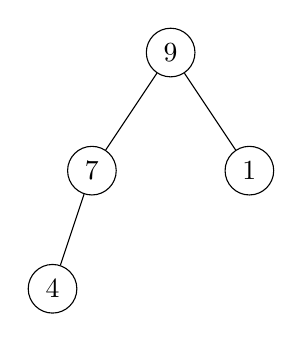
\begin{tikzpicture}[-, level/.style={sibling distance = 2cm/#1, level distance = 1.5cm}, scale=1,transform shape]
    \node[circle,draw](z){$9$}
        child{
            node[circle,draw]{7}
            child{
                node[circle,draw] {4}
                child[missing]
            }
            child[missing]
        }
        child{
            node[circle,draw]{1}
            child[missing]
        };
\end{tikzpicture}
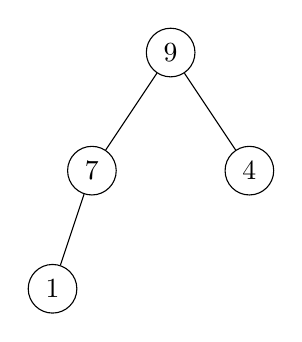
\begin{tikzpicture}[-, level/.style={sibling distance = 2cm/#1, level distance = 1.5cm}, scale=1,transform shape]
    \node[circle,draw](z){$9$}
        child{
            node[circle,draw]{7}
            child{
                node[circle,draw] {1}
                child[missing]
            }
            child[missing]
        }
        child{
            node[circle,draw]{4}
            child[missing]
        };
\end{tikzpicture}
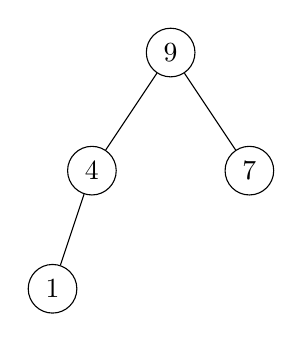
\begin{tikzpicture}[-, level/.style={sibling distance = 2cm/#1, level distance = 1.5cm}, scale=1,transform shape]
    \node[circle,draw](z){$9$}
        child{
            node[circle,draw]{4}
            child{
                node[circle,draw] {1}
                child[missing]
            }
            child[missing]
        }
        child{
            node[circle,draw]{7}
            child[missing]
        };
\end{tikzpicture}
\end{center}

\section*{Exercise 2.}
Given the heap below:
\begin{enumerate}
\item insert $11$
\item remove $14$
\end{enumerate}

% \begin{figure}[h!]
% \centering
% \includegraphics[width=6.5cm]{img/heap-q3.PNG}
% \caption{Heap of Exercise 2.}
% \end{figure}

\subsection*{Solutions exercise 2}
\paragraph{Inserting 11:}{
Insertion of a value will place it on the first free position in the leaves. This is the position below 7 and right of 1. Since this is a max heap, we will have to make sure the children of a node are smaller than itself. This is now not the case, because 7 has a bigger child 11. This problem can be solved by swapping the two nodes. When we check the new parent of 11, we see that this is 16 and since this is bigger, we have the max-heap.
    \begin{center}
    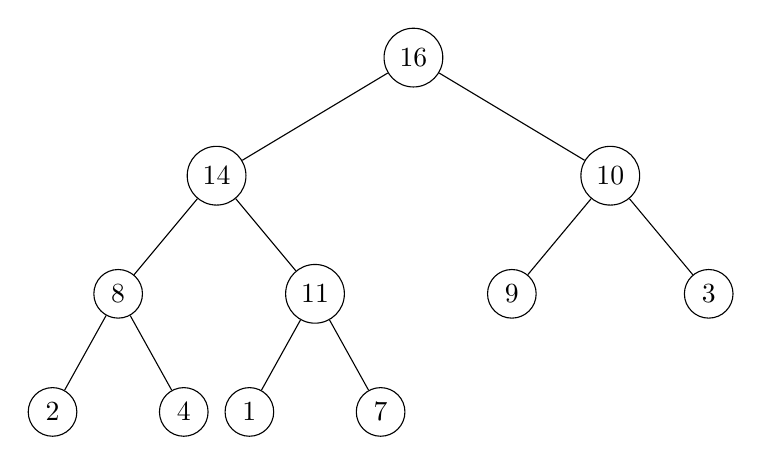
\begin{tikzpicture}[-, level/.style={sibling distance = 5cm/#1, level distance = 1.5cm}, scale=1,transform shape]
    \node[circle,draw](z){$16$}
        child{
            node[circle,draw]{14}
            child{
                node[circle,draw] {8}
                child {
                    node[circle,draw]{2}
                }
                child {
                    node[circle,draw]{4}
                }
            }
            child {
                node[circle,draw]{11}
                child {
                    node[circle,draw]{1}
                }
                child {
                    node[circle,draw]{7}
                }
            }
        }
        child{
            node[circle,draw]{10}
            child{
                node[circle,draw] {9}
            }
            child {
                node[circle,draw] {3}
            }
        };
    \end{tikzpicture}
    \end{center}
}
\
\paragraph{Removing 14:}
Assuming that the steps will take place after each other, we will remove the 14 from the tree which we get after the insertion of 11. Removal of node 14, will take the last node of the leaves to replace it. This is 7. After checking it's children we find out that 7 has a child 11, which conflicts in the heap. After swapping the 7 and 11, we check the parent of 11 and see that this is higher than 11. After that we check the children of 11 and 7, where we see that all children are lower and the max-heap is restored.
\begin{center}
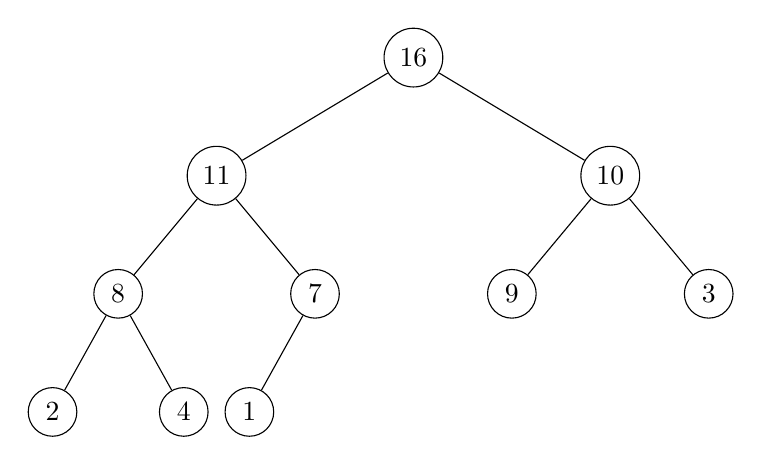
\begin{tikzpicture}[-, level/.style={sibling distance = 5cm/#1, level distance = 1.5cm}, scale=1,transform shape]
\node[circle,draw](z){$16$}
    child{
        node[circle,draw]{11}
        child{
            node[circle,draw] {8}
            child {
                node[circle,draw]{2}
            }
            child {
                node[circle,draw]{4}
            }
        }
        child {
            node[circle,draw]{7}
            child {
                node[circle,draw]{1}
            }
            child[missing]
        }
    }
    child{
        node[circle,draw]{10}
        child{
            node[circle,draw] {9}
        }
        child {
            node[circle,draw] {3}
        }
    };
\end{tikzpicture}
\end{center}

\newpage
\section*{Exercise 3.}
Apply Dijkstra's algorithm on the following graph:
% \begin{figure}[h!]
% \centering
% \includegraphics[width=5cm]{img/dijkstra-1.PNG}
% \caption{Graph of Exercise 3.}
% \end{figure}

\subsection*{Solutions exercise 3}
The solution is shown in the table below. In the solution I assumed that the start vertex for Dijkstra was vertex 0, because the start vertex hasn't been given. The header of the table contains the vertices in the order as they are finished in the queue.
\begin{table}[h]
\centering
\caption{Dijkstra}
\label{my-label}
\begin{tabular}{lllllll}
\hline
Q: & 0 & 1        & 2        & 3        & 4        & 5        \\ \hline
& 0 & $\infty$ & $\infty$ & $\infty$ & $\infty$ & $\infty$ \\
&   & 30       & 40       & $\infty$ & $\infty$ & $\infty$ \\
&   &          & 40       & 50       & 70       & $\infty$ \\
&   &          &          & 50       & 70       & $\infty$ \\
&   &          &          &          & 70       & 110      \\
&   &          &          &          &          & 110
\end{tabular}
\end{table}

\newpage
\section*{Exercise 4.}
Why Dijkstra's algorithm is not working with edges with negative weights? Give an example.

\subsection*{Solutions exercise 4}
We will take the following graph with one negative vertex as example in this solution:
\begin{center}
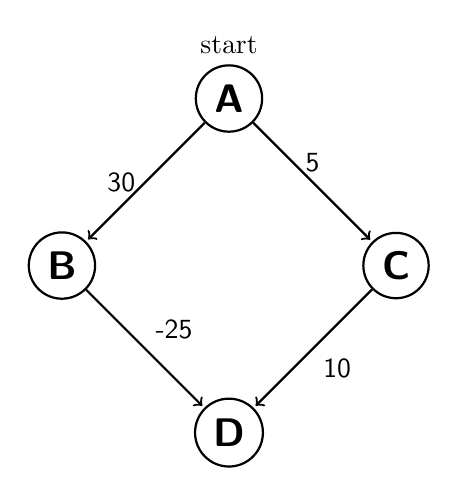
\begin{tikzpicture}[->,shorten >=1pt,auto,node distance=3cm, every loop/.style={},
                    thick, ,main node/.style={circle,draw,font=\sffamily\Large\bfseries}]

  \node[fill = white, text = black, label = start][main node] (1) {A};
  \node[fill = white, text = black][main node] (2) [below left of=1] {B};
  \node[fill = white, text = black][main node] (3) [below right of=1] {C};
  \node[fill = white, text = black][main node] (4) [below right of=2] {D};

  \path[every node/.style={font=\sffamily\normalsize}]
    (1) edge[black] node [left] {30} (2)
        edge[black] node [above] {5} (3)
    (2) edge[black] node {-25} (4)
    (3) edge[black] node {10} (4);
\end{tikzpicture}
\end{center}
% We will use Dijkstra to find the shortest path in this graph for D. This vertex can be reached by the paths A-C-D and path A-B-D. We see that path A-C-D has a cost of 15. When we compare this with the path A-B-D we will see that this total cost is 5. Since the Dijkstra algorithms returns the value of the shortest path, the cost of D will be 5. But for A to B which is a part of A-B-D the cost is 30. In this case we already crossed a longer path than the total length of path A-C-D in total, so this can't the shortest path, since a part is already longer than the total of another path. Dijkstra will not work here, because it will give the wrong path as shortest path.

The Dijkstra algorithm doesn't look anymore to vertices after their neighbours have already been visited. The reason for this is that the algorithm doesn't waste time on paths that are probably longer than the shortest path to the node. When we found a path and 'finish' the vertex, then we cannot specify a new shortest path. \\
So, in the example we will start by giving A the distance 0. From A we will discover it's neighbours B and C, which have lengths 30 and 5. Since the path to C is shorter, we will first do this path. From C we will find the neighbour D which has a total length of 15. We currently have B and D in the queue. Since D has a lower length, we will first discover D further and see that is has no neighbours. We will finish D. We will continue with the last value of the queue, namely B. We see that is has the neighbour D, but this neighbour is already closed because already found the 'shortest' path to it. We This means we won't be able to change the value of the shortest path for D which will remain 15 instead of the actual shortest path of $30 - 25 = 5$. So, in this case Dijkstra will give a longer path for D than the actual shortest path.
\newpage
\section*{Exercise 5.}

% \begin{figure}[h!]
% \centering
% \hspace*{-3cm}
% \includegraphics[width=18cm]{img/dijkstra-map.png}
% \caption{Airlines network.}
% \end{figure}

Airlines companies sell to travelers flights with or without connections, mostly depending on their airlines network.
It can happen that secondary airlines are covered with small and slow aircrafts, hence a longer transit time.
It can then be faster to fly via another city (connecting flight) rather than taking a direct flight, but that's not always the case.
As connections are unpleasant, direct flights are preferred if the total flight time is equal. Otherwise, if the direct flight takes longer, then the connecting flight is preferred.

Let us define $easiest[destination] =$ minimum number of successive flights in a shortest path from $origin$  to  destination.
\newline

In our airlines example, the $easiest$ values are (for origin Madrid):
\begin{itemize}
	\item 0 for Madrid.
	\item 1 for Amsterdam, Berlin, Rome.
	\item 2 for Stockholm, Kiev.
	\item 3 for Moscow.
\end{itemize}

We can transform the problem of the airline company into a graph problem. Give an efficient algorithm taking as input a weighted graph $G = (V,E)$ and a source vertex $s$, and as output the values of $easiest$ for all vertices.

\subsection*{Solutions exercise 5}
We can use Dijkstra to calculate the shortest path for all flights. In order to make the algorithm also keep track of number of flights on the shortest path, we have to add an array with the easiest values for all vertices. If the value of easiest is 1 for a destination, then there is a direct flight, otherwise we took a connective flight.

The easiest of a destination can be calculated by incrementing 1 to the easiest of the easiest of the city where the flight departs.

Another rule was that direct flights are more preferable than connected flights if the flight time is equal. This means we have to add a check whether the flight times are equal. In this check we should check the current easiest of the destination. If this is greater than the easiest of the departure + 1, we have found a direct flight with the same flight time for the destination.

This modified algorithm of Dijkstra can be found below.
\begin{algorithm}[ht!]
  \DontPrintSemicolon

    \Proc{ \dijkstraAirlines{G, s}}{
    $d[s] \leftarrow 0$ \;
    $easiest[s] \leftarrow 0$ \;

    \ForEach{$v \in G[V] - {s}$}{
        $d[s] \leftarrow \infty$ \;
        $easiest[s] \leftarrow \infty$ \;
    }

    $S \leftarrow \oslash $ \;
    $Q \leftarrow V$ \;
    \While{$Q \neq \oslash$}{
        $u \leftarrow$ Extract-min(Q) \;
        $S \leftarrow S \cup \{u \}$ \;
        \ForEach{$v \in Adj[u]$}{
            \If{$d[v] > d[u] + w(u, v)$}{
                $d[v] \leftarrow d[u] + w(u, v)$ \;
                $easiest[v] \leftarrow easiest[u] + 1$ \;
            } \ElseIf{$d[v] = d[u] + w(u, v)$}{
                \If{$easiest[v] > easiest[u] + 1$}{
                    $easiest[v] \leftarrow easiest[u] + 1$ \;
                }
            }
        }
    }

    \KwRet{$easiest$}

  }


    \caption{Easiest for all airlines}
\end{algorithm}


\end{document}
